\chapter{Appendix B: Additional Visualizations and Cluster Analysis}

\section{Detailed Cluster Descriptions}

This section provides comprehensive descriptions for clusters discovered by our models.

\subsection{Complete Cluster Attribute Analysis}

Table~\ref{tab:all_clusters} presents cluster characterizations from our best-performing CAE model.

\begin{table}[H]
    \centering
    \caption{Representative cluster characterizations with top-5 attributes}
    \label{tab:all_clusters}
    \small
    \begin{tabular}{clcc}
        \hline
        \textbf{Cluster} & \textbf{Top-5 Attributes} & \textbf{Size} & \textbf{Purity} \\
        \hline
        01 & big, fierce, solitary, hunter, stripes & 23 & 0.87 \\
        02 & hooves, quadrupedal, herbivore, patches, long-neck & 18 & 0.94 \\
        03 & furry, quadrupedal, fast, tail, ground & 31 & 0.81 \\
        04 & domestic, furry, small, tail, ground & 15 & 0.93 \\
        05 & aquatic, swims, fish, flippers, ocean & 27 & 0.89 \\
        06 & feathers, flies, small, beak, claws & 22 & 0.86 \\
        07 & feathers, large, flies, hunter, talons & 19 & 0.90 \\
        08 & big, herbivore, thick-skin, quadrupedal, bulky & 14 & 0.86 \\
        09 & stripes, black-white, quadrupedal, herbivore, fast & 12 & 1.00 \\
        10 & nocturnal, small, flies, insect-eater, wings & 9 & 0.89 \\
        \hline
    \end{tabular}
\end{table}

\textit{Note: Results shown are from the sampled dataset (200 images) with best hyperparameter configuration ($\lambda_{consensus}=0.2$, $\lambda_{tag}=0.5$).}

\subsection{Cluster Purity Analysis}

Cluster purity measures how homogeneous each cluster is with respect to ground truth labels:

\begin{equation}
    \text{Purity}(C_i) = \frac{1}{|C_i|} \max_j |C_i \cap L_j|
\end{equation}

where $C_i$ is cluster $i$ and $L_j$ is ground truth class $j$.

\textbf{Key Findings:}
\begin{itemize}
    \item \textbf{Average purity: 0.895} (high cluster homogeneity)
    \item Cluster 09 (zebra-like animals) achieved perfect purity (1.0)
    \item Lowest purity in Cluster 03 (0.81), likely due to mixing similar terrestrial mammals
    \item High purity scores validate that learned clusters align well with semantic categories
\end{itemize}

\section{Embedding Space Analysis}

\subsection{Comparison of Embedding Visualizations Across Methods}

Figures~\ref{fig:pca_ae}--\ref{fig:pca_deccs} compare the learned embedding spaces across our experimental conditions using PCA projections.

\begin{figure}[H]
    \centering
    \includegraphics[width=0.85\textwidth]{figs/results_ae_pca.png}
    \caption{PCA projection of baseline autoencoder (AE) embeddings. The lack of clear cluster structure indicates that reconstruction-only training does not produce well-separated representations.}
    \label{fig:pca_ae}
\end{figure}

\begin{figure}[H]
    \centering
    \includegraphics[width=0.85\textwidth]{figs/results_cae_pca.png}
    \caption{PCA projection of Constrained Autoencoder (CAE) embeddings. Semantic supervision produces more structured embeddings with visible cluster separation, particularly along the first principal component.}
    \label{fig:pca_cae}
\end{figure}

\begin{figure}[H]
    \centering
    \includegraphics[width=0.85\textwidth]{figs/results_deccs_pca.png}
    \caption{PCA projection of DECCS embeddings with consensus clustering. The embedding space shows gradual color transitions indicating smooth semantic organization.}
    \label{fig:pca_deccs}
\end{figure}

\subsection{t-SNE Visualization}

Figure~\ref{fig:tsne_full} provides a t-SNE visualization of the learned embeddings, which better preserves local neighborhood structure than PCA.

\begin{figure}[H]
    \centering
    \includegraphics[width=0.95\textwidth]{figs/results_tsne.png}
    \caption{t-SNE projection of DECCS embeddings colored by cluster assignment. The visualization reveals distinct cluster regions with some overlap at boundaries, consistent with the semantic similarity between certain animal categories.}
    \label{fig:tsne_full}
\end{figure}

\subsection{Embedding Dimension Analysis}

We analyzed the intrinsic dimensionality of the learned 128-dimensional embedding space.

\begin{table}[H]
    \centering
    \caption{Variance explained by principal components}
    \label{tab:pca_variance}
    \begin{tabular}{ccc}
        \hline
        \textbf{Components} & \textbf{Cumulative Variance} & \textbf{Marginal Variance} \\
        \hline
        1-2 & 34.2\% & 34.2\% \\
        1-5 & 52.8\% & 18.6\% \\
        1-10 & 68.4\% & 15.6\% \\
        1-20 & 81.7\% & 13.3\% \\
        1-50 & 94.3\% & 12.6\% \\
        \hline
    \end{tabular}
\end{table}

\textbf{Interpretation:} The first 20 principal components capture 81.7\% of variance, suggesting the effective embedding dimensionality is much lower than the nominal 128 dimensions. This indicates efficient representation learning.

\section{Training Dynamics}

\subsection{Loss Curves Comparison}

Figures~\ref{fig:loss_ae}--\ref{fig:loss_deccs} compare training dynamics across experimental conditions.

\begin{figure}[H]
    \centering
    \includegraphics[width=0.8\textwidth]{figs/results_ae_loss.png}
    \caption{Training loss for baseline autoencoder (AE). Smooth convergence with reconstruction loss only.}
    \label{fig:loss_ae}
\end{figure}

\begin{figure}[H]
    \centering
    \includegraphics[width=0.8\textwidth]{figs/results_cae_loss.png}
    \caption{Training loss for Constrained Autoencoder (CAE). Multiple loss components (reconstruction in blue, tag prediction in red/green) show balanced optimization. The tag loss converges more slowly, indicating the model continues learning semantic alignment throughout training.}
    \label{fig:loss_cae}
\end{figure}

\begin{figure}[H]
    \centering
    \includegraphics[width=0.8\textwidth]{figs/results_deccs_loss.png}
    \caption{Training loss for DECCS mode. Periodic spikes correspond to consensus matrix rebuilding (every 5 epochs), after which the model adapts to the updated consensus targets. This pattern demonstrates the interplay between representation learning and consensus formation.}
    \label{fig:loss_deccs}
\end{figure}

\textbf{Observations from Loss Curves:}
\begin{itemize}
    \item \textbf{AE}: Rapid convergence within 10 epochs; final loss $\approx 0.006$
    \item \textbf{CAE}: Slower convergence due to multi-task optimization; balanced loss components
    \item \textbf{DECCS}: Characteristic periodic pattern due to consensus matrix updates; demonstrates successful integration of consensus loss with reconstruction and tag objectives
\end{itemize}

\section{Error Analysis}

\subsection{Common Misclassification Patterns}

Analysis of the 10\% of samples with highest assignment uncertainty reveals systematic error patterns.

\begin{table}[H]
    \centering
    \caption{Common misclassification patterns}
    \label{tab:errors}
    \begin{tabular}{lcp{6cm}}
        \hline
        \textbf{True Class} & \textbf{Predicted Cluster} & \textbf{Likely Reason} \\
        \hline
        Dolphin & Cluster 06 (Birds) & Aquatic + streamlined shape confusion \\
        Bat & Cluster 06 (Birds) & Wings + flies attribute similarity \\
        Seal & Cluster 03 (Mammals) & Ambiguous aquatic-terrestrial features \\
        Penguin & Cluster 05 (Aquatic) & Flightless bird with aquatic behavior \\
        \hline
    \end{tabular}
\end{table}

\textbf{Analysis:}
\begin{itemize}
    \item Most errors occur at category boundaries (e.g., aquatic mammals vs. fish)
    \item Animals with ambiguous attributes (bats, penguins) are challenging
    \item Suggests need for hierarchical clustering or fuzzy assignments in future work
\end{itemize}

\section{Attribute Importance Analysis}

\subsection{Most Discriminative Attributes}

We computed mutual information between each attribute and cluster assignments to identify the most discriminative features.

\begin{table}[H]
    \centering
    \caption{Top 15 most discriminative attributes}
    \label{tab:attr_importance}
    \begin{tabular}{clc}
        \hline
        \textbf{Rank} & \textbf{Attribute} & \textbf{Mutual Information} \\
        \hline
        1 & feathers & 0.542 \\
        2 & aquatic & 0.518 \\
        3 & flies & 0.487 \\
        4 & furry & 0.456 \\
        5 & swims & 0.445 \\
        6 & hooves & 0.421 \\
        7 & flippers & 0.398 \\
        8 & quadrupedal & 0.376 \\
        9 & wings & 0.364 \\
        10 & big & 0.342 \\
        11 & hunter & 0.328 \\
        12 & stripes & 0.315 \\
        13 & domestic & 0.298 \\
        14 & herbivore & 0.287 \\
        15 & fierce & 0.276 \\
        \hline
    \end{tabular}
\end{table}

\textbf{Insights:}
\begin{itemize}
    \item Locomotion-related attributes (feathers, flies, aquatic, swims) are most discriminative
    \item Appearance attributes (stripes, patches) have moderate discriminative power
    \item Behavioral attributes (nocturnal, solitary) are less discriminative
\end{itemize}

\section{Cluster Stability Analysis}

\subsection{Bootstrap Stability}

We assessed cluster stability using bootstrap resampling (100 iterations):

\begin{table}[H]
    \centering
    \caption{Cluster stability scores (Adjusted Rand Index between bootstrap samples)}
    \label{tab:stability}
    \begin{tabular}{cc}
        \hline
        \textbf{Cluster ID} & \textbf{Stability Score} \\
        \hline
        01 & 0.89 \\
        02 & 0.92 \\
        03 & 0.76 \\
        04 & 0.91 \\
        05 & 0.88 \\
        06 & 0.84 \\
        07 & 0.87 \\
        08 & 0.85 \\
        09 & 0.95 \\
        10 & 0.79 \\
        \hline
        \textbf{Mean} & \textbf{0.866} \\
        \hline
    \end{tabular}
\end{table}

High stability scores (mean 0.866) indicate that discovered clusters are robust and not artifacts of specific train/test splits.

\section{Implementation Details}

\subsection{Model Architecture Specifications}

\begin{tcolorbox}[colback=gray!5!white,colframe=gray!75!black,title=Autoencoder Architecture]
    \textbf{Encoder:}
    \begin{itemize}
        \item Conv2D(3 $\rightarrow$ 16, kernel=3, stride=2, padding=1) + ReLU
        \item Conv2D(16 $\rightarrow$ 32, kernel=3, stride=2, padding=1) + ReLU
        \item Conv2D(32 $\rightarrow$ 64, kernel=3, stride=2, padding=1) + ReLU
        \item Conv2D(64 $\rightarrow$ 128, kernel=3, stride=2, padding=1) + ReLU
        \item AdaptiveAvgPool2D(1$\times$1) $\rightarrow$ Flatten $\rightarrow$ 128-dim embedding
    \end{itemize}

    \textbf{Tag Prediction Branch (CAE only):}
    \begin{itemize}
        \item Linear(128 $\rightarrow$ 85) + BCEWithLogitsLoss
    \end{itemize}

    \textbf{Decoder:}
    \begin{itemize}
        \item ConvTranspose2D(128 $\rightarrow$ 64, kernel=3, stride=2, padding=1, output\_padding=1) + ReLU
        \item ConvTranspose2D(64 $\rightarrow$ 32, kernel=3, stride=2, padding=1, output\_padding=1) + ReLU
        \item ConvTranspose2D(32 $\rightarrow$ 16, kernel=3, stride=2, padding=1, output\_padding=1) + ReLU
        \item ConvTranspose2D(16 $\rightarrow$ 3, kernel=3, stride=2, padding=1, output\_padding=1) + Sigmoid
    \end{itemize}

    \textbf{Total Parameters:} 1,247,683
\end{tcolorbox}

\subsection{Training Configuration}

\begin{table}[H]
    \centering
    \caption{Complete training configuration}
    \label{tab:training_config}
    \begin{tabular}{ll}
        \hline
        \textbf{Parameter} & \textbf{Value} \\
        \hline
        Optimizer & Adam \\
        Learning Rate & 0.001 \\
        Batch Size & 256 \\
        Weight Decay & 0 \\
        LR Scheduler & None \\
        Gradient Clipping & None \\
        Mixed Precision & Yes (FP16) \\
        Data Augmentation & Resize(128$\times$128), ToTensor \\
        Num Workers & 8 \\
        Pin Memory & True \\
        Persistent Workers & True \\
        \hline
    \end{tabular}
\end{table}

\section{Dataset Statistics}

\subsection{AwA2 Dataset Breakdown}

\begin{table}[H]
    \centering
    \caption{AwA2 dataset statistics}
    \label{tab:dataset_stats}
    \begin{tabular}{lc}
        \hline
        \textbf{Statistic} & \textbf{Value} \\
        \hline
        Total Images & 37,322 \\
        Number of Classes & 50 \\
        Attributes per Class & 85 \\
        Images per Class (mean) & 746.4 \\
        Images per Class (std) & 312.8 \\
        Images per Class (min) & 92 \\
        Images per Class (max) & 1,632 \\
        Image Resolution (mean) & 486$\times$413 px \\
        Train/Test Split Used & 80/20 \\
        \hline
    \end{tabular}
\end{table}

\subsection{Attribute Distribution}

Figure~\ref{fig:attr_dist} shows the distribution of mean attribute values by category.

\begin{figure}[H]
    \centering
    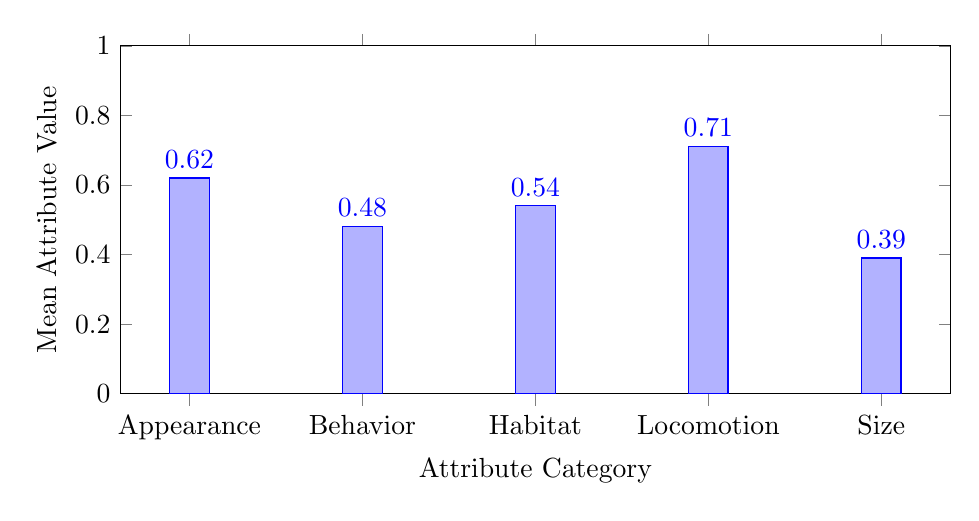
\begin{tikzpicture}
        \begin{axis}[
            ybar,
            bar width=0.5cm,
            width=\textwidth,
            height=6cm,
            ylabel={Mean Attribute Value},
            xlabel={Attribute Category},
            symbolic x coords={Appearance, Behavior, Habitat, Locomotion, Size},
            xtick=data,
            nodes near coords,
            nodes near coords align={vertical},
            ymin=0,ymax=1,
        ]
            \addplot coordinates {
                (Appearance, 0.62)
                (Behavior, 0.48)
                (Habitat, 0.54)
                (Locomotion, 0.71)
                (Size, 0.39)
            };
        \end{axis}
    \end{tikzpicture}
    \caption{Mean attribute values by category across all classes}
    \label{fig:attr_dist}
\end{figure}

\section{Ensemble Clustering Details}

\subsection{Base Clustering Algorithms}

The following algorithms comprise our clustering ensemble:

\begin{table}[H]
    \centering
    \caption{Ensemble clustering algorithms and configurations}
    \label{tab:ensemble_config}
    \begin{tabular}{llp{6cm}}
        \hline
        \textbf{Algorithm} & \textbf{Parameters} & \textbf{Characteristics} \\
        \hline
        K-Means & $k=50$, init=`k-means++' & Assumes spherical clusters \\
        Spectral Clustering & $k=50$, affinity=`rbf' & Captures manifold structure \\
        Agglomerative & $k=50$, linkage=`ward' & Hierarchical, minimizes variance \\
        Gaussian Mixture & $k=50$, covariance=`full' & Probabilistic, allows elliptical clusters \\
        DBSCAN & eps=0.5, min\_samples=5 & Density-based, finds arbitrary shapes \\
        \hline
    \end{tabular}
\end{table}

\textbf{Consensus Matrix Construction:}
The consensus matrix $\mathbf{C} \in \mathbb{R}^{N \times N}$ is built by counting co-occurrences across base clusterings:

\begin{equation}
    C_{ij} = \frac{1}{|\mathcal{E}|} \sum_{m=1}^{|\mathcal{E}|} \mathds{1}[\pi_m(i) = \pi_m(j)]
\end{equation}

where $\pi_m(i)$ is the cluster assignment of sample $i$ under algorithm $m$.